\documentclass[fleqn,usenatbib]{mnras}

% MNRAS is set in Times font. If you don't have this installed (most LaTeX
% installations will be fine) or prefer the old Computer Modern fonts, comment
% out the following line
%\usepackage{newtxtext,newtxmath}
\usepackage{times}
% Depending on your LaTeX fonts installation, you might get better results with one of these:
% \usepackage{mathptmx}
% \usepackage{txfonts}

% Use vector fonts, so it zooms properly in on-screen viewing software
% Don't change these lines unless you know what you are doing
\usepackage[T1]{fontenc}
\usepackage{ae,aecompl}


%%%%% AUTHORS - PLACE YOUR OWN PACKAGES HERE %%%%%
%\usepackage{epsf}
\usepackage{color}
\usepackage{graphicx}
\usepackage{amsmath}	% Advanced maths commands
\usepackage{amssymb}	% Extra maths symbols
\usepackage{mathrsfs}	% Extra extra math symbols
\usepackage{natbib}
%\usepackage[colorlinks,urlcolor=magenta,citecolor=blue,linkcolor=blue]{hyperref}
\usepackage{multirow}
\usepackage{etoolbox}
\usepackage{listings}

\graphicspath{{./figures/}}

%%%%% AUTHORS - PLACE YOUR OWN COMMANDS HERE %%%%%
%%% Fields %%%
\newcommand{\hdf}{HDF-N}
\newcommand{\hdfn}{HDF-N}
\newcommand{\hdfs}{HDF-S}
\newcommand{\cdfs}{CDF-S}

%%% Telescopes %%%
\newcommand{\hst}{\textit{HST}}
\newcommand{\iras}{\textit{IRAS}}
\newcommand{\iso}{\textit{ISO}}
\newcommand{\spitzer}{\textit{Spitzer}}
\newcommand{\sirtf}{\textit{Spitzer}}
\newcommand{\chandra}{\textit{Chandra}}

%%% Filters %%%
\newcommand{\wfu}{\hbox{$\mathrm{U}_{300}$}}
\newcommand{\wfb}{\hbox{$\mathrm{B}_{450}$}}
\newcommand{\wfv}{\hbox{$\mathrm{V}_{606}$}}
\newcommand{\wfi}{\hbox{$\mathrm{I}_{814}$}}
\newcommand{\acsb}{\hbox{$\mathrm{B}_{435}$}}
\newcommand{\acsv}{\hbox{$\mathrm{V}_{606}$}}
\newcommand{\acsi}{\hbox{$i_{775}$}}
\newcommand{\acsz}{\hbox{$z_{850}$}}
\newcommand{\nicj}{\hbox{$\mathrm{J}_{110}$}}
\newcommand{\nich}{\hbox{$\mathrm{H}_{160}$}}
\newcommand{\wfcy}{\hbox{$\mathrm{Y}_{105}$}}
\newcommand{\wfcj}{\hbox{$\mathrm{J}_{125}$}}
%\newcommand{\wfcj}{\hbox{$J_{110}$}}
\newcommand{\wfch}{\hbox{$\mathrm{H}_{160}$}}
\newcommand{\sdssu}{\hbox{$u$}}
\newcommand{\sdssg}{\hbox{$g$}}
\newcommand{\sdssr}{\hbox{$r$}}
\newcommand{\sdssi}{\hbox{$i$}}
\newcommand{\sdssz}{\hbox{$z$}}
\newcommand{\mone}{\hbox{$[3.6]$}}
\newcommand{\mtwo}{\hbox{$[4.5]$}}
\newcommand{\mthree}{\hbox{$[5.8]$}}
\newcommand{\mfour}{\hbox{$[8.0]$}}
%\newcommand{\mone}{\hbox{$[3.6\mu\mathrm{m}]$}}
%\newcommand{\mtwo}{\hbox{$[4.5\mu\mathrm{m}]$}}
%\newcommand{\mthree}{\hbox{$[5.8\mu\mathrm{m}]$}}
%\newcommand{\mfour}{\hbox{$[8.0\mu\mathrm{m}]$}}

%%% Astronomy Abreviations %%%
\newcommand{\mstar}{\hbox{$\mathrm{M}^\ast$}}
\newcommand{\lstar}{\hbox{$L^\ast$}}
\newcommand{\Msol}{\hbox{$\mathrm{M}_\odot$}}
\newcommand{\msol}{\hbox{$\mathrm{M}_\odot$}}
\newcommand{\Zsol}{\hbox{$Z_\odot$}}
\newcommand{\zsol}{\hbox{$Z_\odot$}}
\newcommand{\Lsol}{\hbox{$L_\odot$}}
\newcommand{\lsol}{\hbox{$L_\odot$}}
\newcommand{\lir}{\hbox{$L_{\mathrm{IR}}$}}
\newcommand{\zph}{\hbox{$z_\mathrm{ph}$}}
\newcommand{\zphot}{\hbox{$z_\mathrm{ph}$}}
\newcommand{\lbol}{\hbox{$L_\mathrm{bol}$}}
\newcommand{\snr}{\hbox{$\mathrm{S/N}$}}
\newcommand{\reff}{\hbox{$r_\mathrm{eff}$}}
\newcommand{\ks}{\hbox{$K_s$}}
\newcommand{\AAA}{\hbox{\AA}}

%%% Spectrum Lines %%%
\newcommand{\lya}{ Ly$\alpha \;$}
\newcommand{\lyb}{Lyman~$\beta$}
\newcommand{\hb}{\hbox{H$\beta$}}
\newcommand{\ha}{\hbox{H$\alpha$}}
\newcommand{\paa}{\hbox{Pa$\alpha$}}

%%% Units %%%
\newcommand{\kms}{\hbox{km~s$^{-1}$}}
\newcommand{\cms}{\hbox{cm~s$^{-1}$}}
\newcommand{\mpc}{\hbox{Mpc$^{-1}$}}
\newcommand{\mpcsq}{\hbox{Mpc$^{-2}$}}
\newcommand{\mpccu}{\hbox{Mpc$^{-3}$}}
\newcommand{\cnts}{\hbox{cnt~s$^{-1}$}} 
\newcommand{\cmsq}{\hbox{cm$^{-2}$}}
\newcommand{\cmcu}{\hbox{cm$^{-3}$}}
\newcommand{\ergscm}{\hbox{erg~s$^{-1}$~cm$^{-2}$}}
\newcommand{\uJy}{\hbox{$\mu$Jy}}
\newcommand{\ujy}{\hbox{$\mu$Jy}}
\newcommand{\degree}{\hbox{$^\circ$}}
\newcommand{\degsq}{\hbox{degree$^2$}}
\newcommand{\arcminsq}{\hbox{arcmin$^2$}}
\newcommand{\um}{\hbox{$\mu$m}}

%%% Math %%%
\newcommand{\lsim}{\lesssim}
\newcommand{\gsim}{\gtrsim}
\newcommand{\mathS}{\hbox{$\mathcal{S}$}}
\newcommand{\mathR}{\hbox{$\mathcal{R}$}}
\newcommand{\mathM}{\hbox{$\mathcal{M}$}}
\newcommand{\mcal}{\hbox{$\mathcal{M}$}}
\newcommand{\rcal}{\hbox{$\mathcal{R}$}}
\newcommand{\scal}{\hbox{$\mathcal{S}$}}
\newcommand{\infinity}{\hbox{$\infty$}}
\newcommand{\err}[2]{$^{+#2}_{-#1}$}

%%% General %%%
\newcommand{\etal}{et al.}
\newcommand{\eg}{e.g.}
\newcommand{\ie}{i.e.}
\newcommand{\cf}{cf.}
% \newcommand{\ion}[2]{\hbox{#1$\;${\small\rm{#2}}}}
\newcommand{\mybullet}{\noindent$\bullet$}
\newcommand{\uit}{\textit{UIT}}
\newcommand{\nd}{...}
%\newcommand{\cmodel}{\hbox{\tt cmodel}}
%\newcommand{\bs}{\hbox{$\!\!\!\!$}}
\newcommand{\todo}[1]{{\tt #1}}
\newcommand{\citeeg}[1]{(\eg, \citealt{#1})}
\newcommand{\ignore}[1]{}

%%% Extra %%% 
% \newcommand{\farcm}{\mbox{\ensuremath{.\mkern-4mu^\prime}}}%fractional arcminute symbol 0.'0
% \newcommand{\farcs}{\mbox{\ensuremath{.\!\!^{\prime\prime}}}}%fractional arcsecond symbol: 0.''0
% \newcommand{\fdg}{\mbox{\ensuremath{.\!\!^\circ}}}%fractional degree symbol:     0.°0
\newcommand{\arcdeg}{\ensuremath{^{\circ}}}%                    % degree symbol:  °
% \newcommand{\sun}{\ensuremath{\odot}}%                          % sun symbol
% \newcommand{\apj}{ApJ}%                                         % Journal abbreviations
% \newcommand{\apjs}{ApJS}
% \newcommand{\apjl}{ApJL}
% \newcommand{\aap}{A{\&}A}
% \newcommand{\aaps}{A{\&}AS}
% \newcommand{\mnras}{MNRAS}
% \newcommand{\aj}{AJ}
% \newcommand{\araa}{ARAA}
% \newcommand{\pasp}{PASP}
\newcommand{\Teff}{\ensuremath{T_{\mathrm{eff}}}}%              % T_eff
\newcommand{\logg}{\ensuremath{\log g}}%                        % log g
\newcommand{\bv}{\ensuremath{B\!-\!V}}%                         % B-V
\newcommand{\ub}{\ensuremath{U\!-\!B}}%                         % U-B
\newcommand{\vr}{\ensuremath{V\!-\!R}}%                         % V-R
\newcommand{\ur}{\ensuremath{U\!-\!R}}%                         % U-R

\newcommand{\editorial}[1]{\textcolor{red}{#1}}
\newcommand{\multic}[2]{\multicolumn{#1}{c}{#2}}
\newcommand{\rottext}[2]{\multirow{#1}{*}{\rotatebox[origin=c]{90}{#2}}}

%%%%%%%%%%%%%%%%%%% TITLE PAGE %%%%%%%%%%%%%%%%%%%
\title[Metallicity with CNNs]{Predicting Galaxy Metallicity from Three-Color Images using Convolutional Neural Networks}

% The list of authors, and the short list which is used in the headers.
% If you need two or more lines of authors, add an extra line using \newauthor
\author[Wu and Boada]
{\parbox{\textwidth}{John~Wu$^{1}$\thanks{E-mail: jw740@physics.rutgers.edu} and
Steven~Boada$^{1}$}\vspace{0.4cm}\
\\
\parbox{\textwidth}{$^{1}$Physics and Astronomy Department, Rutgers University, Piscataway, NJ 08854-8019, USA\\}}

% These dates will be filled out by the publisher
\date{Accepted XXX. Received YYY; in original form ZZZ}

% Enter the current year, for the copyright statements etc.
\pubyear{2018}

% Don't change these lines
\begin{document}
\label{firstpage}
\pagerange{\pageref{firstpage}--\pageref{lastpage}}
\maketitle

\begin{abstract}
\noindent
Lorem ipsum dolor sit amet, consectetur adipisicing elit, sed do eiusmod tempor incididunt ut labore et dolore magna aliqua. Ut enim ad minim veniam, quis nostrud exercitation ullamco laboris nisi ut aliquip ex ea commodo consequat. Duis aute irure dolor in reprehenderit in voluptate velit esse cillum dolore eu fugiat nulla pariatur. Excepteur sint occaecat cupidatat non proident, sunt in culpa qui officia deserunt mollit anim id est laborum.
\end{abstract}

\section{Introduction}\label{sec:introduction}
\editorial{Things we are going to want to talk about in the introduction: Morphology-metalicity relation? There is certainly a mass-metallicity relation. Basically, we want to say why we think we can do this at all? What is the primary science driver behind why we think this will work? Is it really just the fundamental plane? We aren't telling the thing about the mass or the distance to the objects.}
\editorial{I'll add some words we might want to use}
Large-area sky surveys, both on-going and planned, are revolutionizing our understanding of galaxy evolution. The on going Dark Energy Survey (DES; \citealt{DES2005}) and planned Large Synoptic Survey Telescope (LSST; \citealt{LSST2012}) will survey vast swaths of the sky and create samples of galaxies much larger than any previously know. Spectroscopic follow-up will be key to a deep understanding of the properties of these galaxies, and constrain \editorial{something something}. But as the dataset continues to grow individual follow-up becomes increasingly impractical. Therefore, large spectroscopic surveys are needed to more fully understand the observable-mass relation of clusters.
In this work, we propose to use supervised ML, specifically convolution neural networks, to analyze pseudo-three color images to predict galaxy metallicity.
This paper is organized as follows: Section \ref{sec:CNN} we briefly introduce convolutional neural networks, discuss selection of the network's hyperparameters and outline training the network. In Section~\ref{sec:data}, we describe the acquisition and cleaning of the SDSS data sample. We present the main results in Section~\ref{sec:results} and discuss the results in the context of previous works in Section~\ref{sec:discussion}. In Section~\ref{sec:summary}, we summarize the key results and conclude.
Unless otherwise noted, throughout this paper, we use a concordance cosmological model ($\Omega_\Lambda = 0.7$, $\Omega_m = 0.3$, and $H_0= 70$ \kms \mpc), assume a Chabrier initial mass function \citep{Chabrier2003}, and use AB magnitudes \citep{Oke1974}.

\section{Convolutional Neural Networks}\label{sec:CNN}
In recent years, neural networks have been able to accomplish a large number of tasks in the field of machine learning (LeCun et al. 1989).
Image classification and regression problems are most readily solved by use of convolutions in mutliple layers of the network (see, e.g., Krizhevsky et al. 2012).
Convolution neural networks (CNNs, or convnets) efficiently learn spatial relations in images whose features are about the same sizes as the convolution filters (or kernels) which are to be learned through training.
CNNs are considered \textit{deep} when the number of convolutional layers is large; visualizing their filters reveals that increased depth permits the network to learn more and more abstract features (e.g., from Gabor filters, to geometric shapes, to faces; Zeiler \& Fergus 2013).

The input layer is simply an image of $128\times 128$ pixels with three channels (RGB).
Dieleman et al. (Galaxy Zoo Kaggle competition) have already shown that CNNs are capable of classifying the morphologies of such images of galaxies from the Sloan Digital Sky Survey (SDSS) with the same accuracy as citizen scientists.
Other people have been done other cools things (like use simulated images to select real galaxies, etc).
blah blah blah.
Define overfitting: a specific and usually not general set of features are learned and misapplied to the test set data.

We split our training sample of $\sim 130,000$ images into sets of $90,000$ for training, $20,000$ for validation, and $20,000$ for testing.
Training images are seen once every epoch, although usually each epoch is split into a number of mini-batches which are learned in parallel.
Mini-batches are usually small ($256?$) and potentially not representative of the full training sample -- another technique used to prevent overfitting.
Each mini-batch is fed forward through the input layers, where a random fraction of connections $p=0.25, 0.50$ are removed between each linear layer (dropout, Hinton et al. 2012; see subsection below).
When the feed-forward network reports a prediction, whether a single or set of quantities, then a loss/cost function is used to compute how incorrect the prediction ($\hat y$) is from the true value $y$.
We use the root mean squared error (RMSE$~\equiv \sqrt{\langle |\hat y - y|^2\rangle}$) loss function, and seek to minimize it.
We use gradient descent for each mini-batch to adjust each weight parameter, and each fractional contribution of loss is determined by the backpropagation algorithm (cite original, LeCun et al.). 
The backpropagation algorithm is simply the chain rule applied to finite derivatives, and skipped? for any non-linear layers.
The gradient is multiplied by the \textit{learning rate}; batch-normalization is also applied in addition to a momentum term which ensures that the gradient is itself only changing slowly with each mini-batch.


\section{Data and training}\label{sec:data}

\subsection{SDSS images}
Our sample of galaxies are selected from the NYU Value Added Catalog (VAC) \editorial{cite}, to have gas phase metallicities. The metallicity estimates \citep{Tremonti2004} are derived from spectroscopic measurements and for the purposes of this work are assumed to be ``the truth.'' In addition, we take the derived stellar mass for each galaxy.
We supplement the data from the VAC with data from SDSS Data Release 13 (DR13; \citealt{Albareti2017}) for each galaxy, the right ascension and declination and the magnitude in each of the five SDSS photometric bands (\sdssu, \sdssg, \sdssr, \sdssi, \sdssz), along with associated errors. We require that galaxies magnitudes are $10 < \sdssu\sdssg\sdssr\sdssi\sdssz < 25$ mag. Galaxies should have colors $0 < \sdssu-\sdssr < 6$ \editorial{why?}, high confidence ($z_{err} < 0.01$) spectroscopic redshifts greater than $0.2$, \editorial{check the petro mags and why we are using those}.

From this input catalog we create RGB images with the SDSS cutout service\footnote{\url{http://skyserver.sdss.org/dr14/SkyserverWS/ImgCutout/getjpeg}}. Images are scaled to be $128\times128$ pixels in size, corresponding to $15''\times15''$ on the sky. This results in the native $0\farcs396$ pixelscale of the SDSS being rescaled to $0\farcs296$ per pixel.
We create $142,176$ three color images which serve as the main data set for this work.

\subsection{Training in practice}

%It takes under thirty minutes on the same GPU to reach RMSE$~=0.10$ in metallicity.
Our training methods near convergence after 10 epochs, although additional training continue to improve the loss.
In total, the training requires 25-30 minutes on our GPU and uses under 2~GB of memory (depending on batch size).
$k$-fold ensemble methods take $k$ times as long to train.
Prediction using TTA takes two minutes for our full test set of about 20,000 images, or approximately 6~milliseconds per image (or a little over 1~millisecond per image without TTA).
Super-convergent training the network takes about 10 hours on a GPU but only yield marginal improvements over the ensemble methods (RMSE~$= 0.0828$ for super-convergent versus $0.0835$ for 5-fold).




\begin{lstlisting}[language=PYTHON]
lr = 1e-1
learn.fit(lr, 2)

lrs = [1e-3, 1e-2, 1e-1]
learn.unfreeze()
learn.fit(lr, 1)
learn.fit(lr, 3, cycle_len=1, cycle_mult=2)
\end{lstlisting}

In comparison, Huertas-Company et al. 2015 train their network for 10 days on a GPU following the Galaxy Zoo architecture.


We evaluate predictions using not only the RMSE, which approaches the standard deviation for Gaussian-distributed data, but also the NMAD, or the normal median absolute deviation:
\begin{equation}
{\rm NMAD}(x) \approx 1.4826 \times {\rm median} \big (\big|x - {\rm median }(x) \big|\big ),
\end{equation}
where for a Gaussian-distributed $x$, the NMAD will also approximate the standard deviation, $\sigma$.
NMAD is outlier-insensitive for non-Gaussian distributions and is useful for comparing scatter.

\section{Results}\label{sec:results}

See figure for 50th percentile [O/H] predictions.


\begin{figure}
	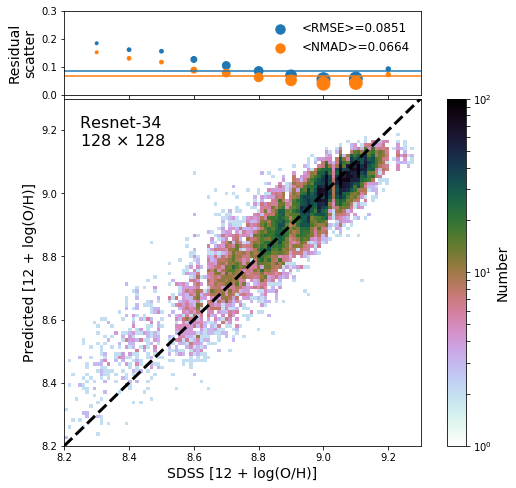
\includegraphics[width=\columnwidth]{predicted-vs-true-metallicity.png}
	\caption{\label{fig:predicting-metallicity}
		Our main result is shown in the main (lower) panel. 
		We show metallicity predictions from \textit{gri} imaging using a 34-layer residual convnet, compared to true metallicities from SDSS (Tremonti et al. 2004).
		In the upper panel, we show the residual, or difference between prediction and truth values, as a function of true metallicity.
		The size of markers is proportional to the number of galaxies in each true metallicity bin.
		The average RMSE and outlier-insensitive NMAD for the entire test set are 0.0851 and 0.0664 respectively, and are shown as horizontal colored lines.}
\end{figure}




\begin{figure}
	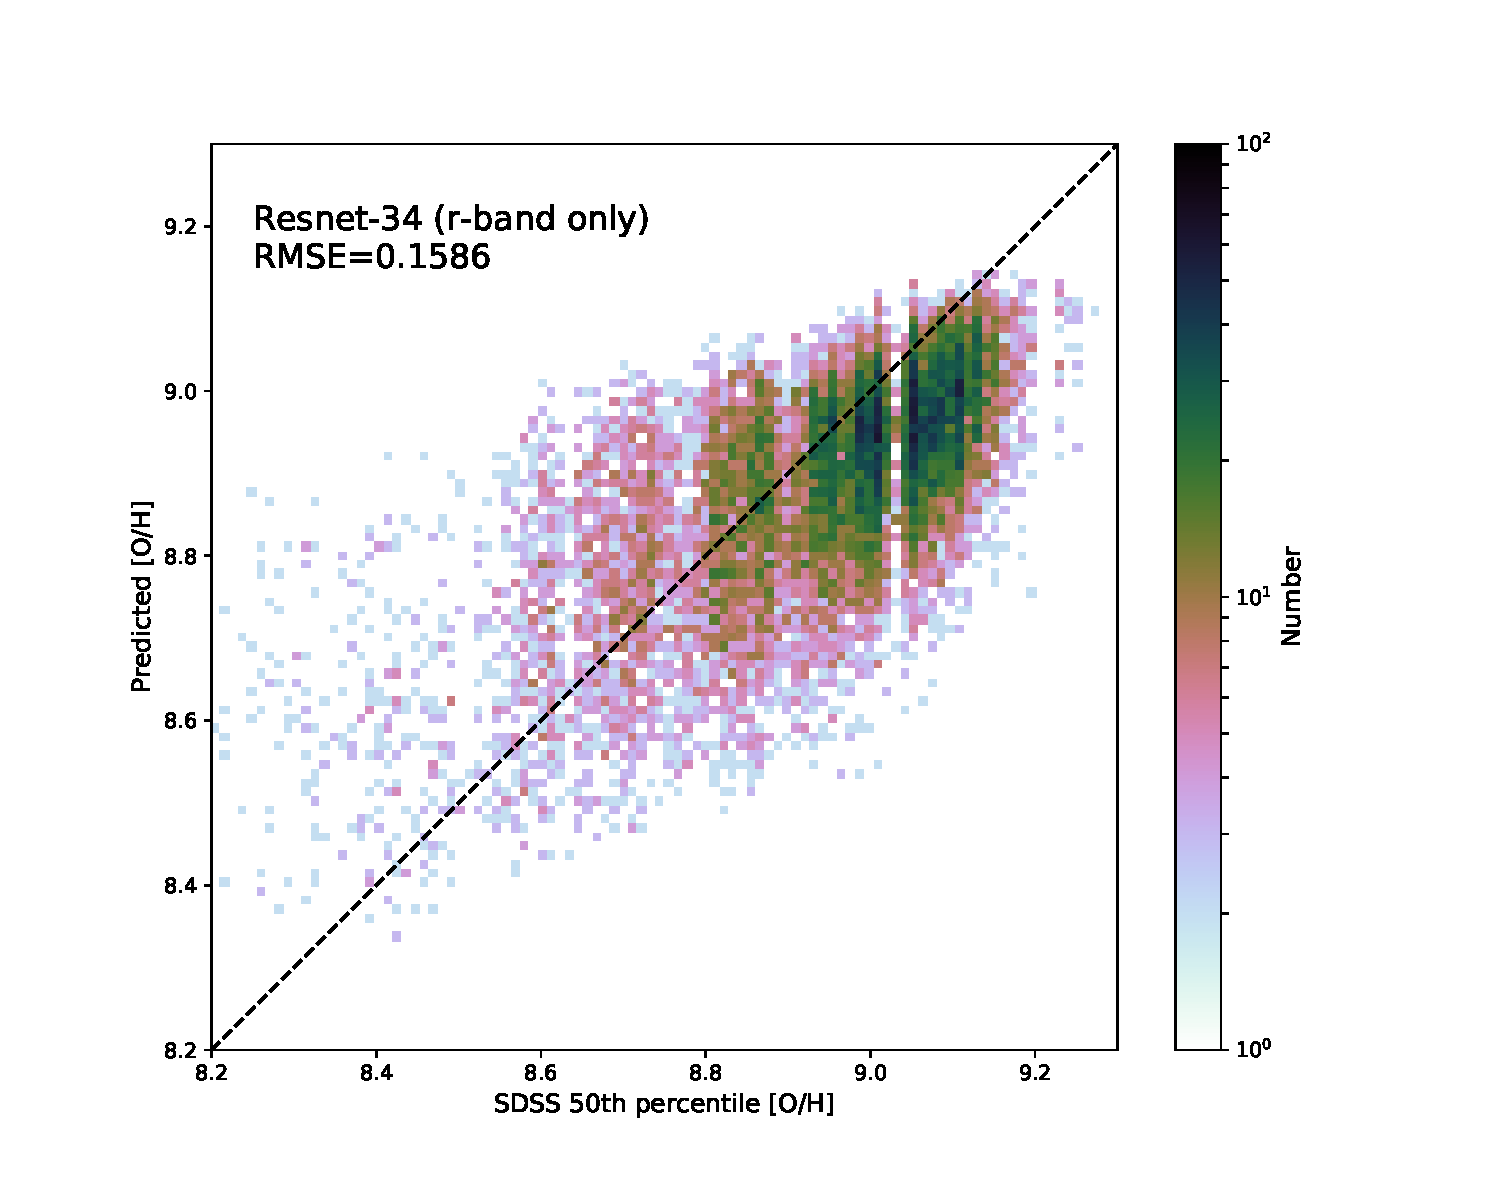
\includegraphics[width=\columnwidth]{r-band_pred-vs-SDSS.pdf}
	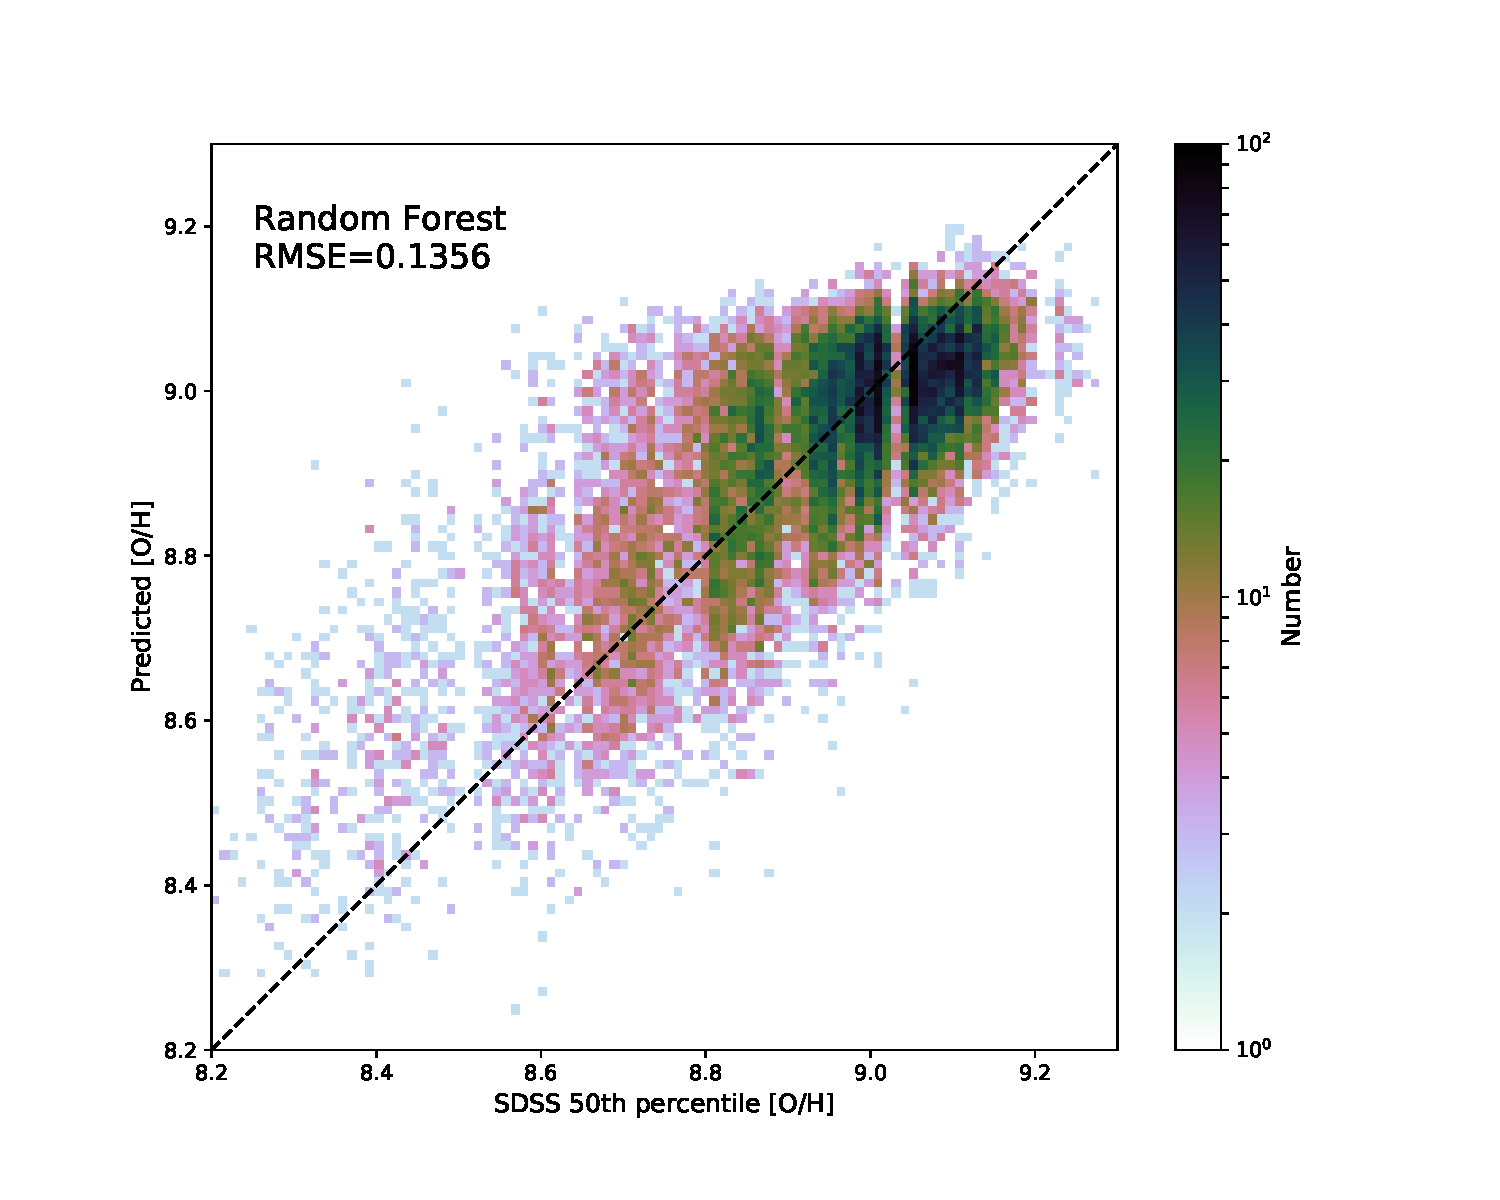
\includegraphics[width=\columnwidth]{random-forest_pred-vs-SDSS.pdf}
	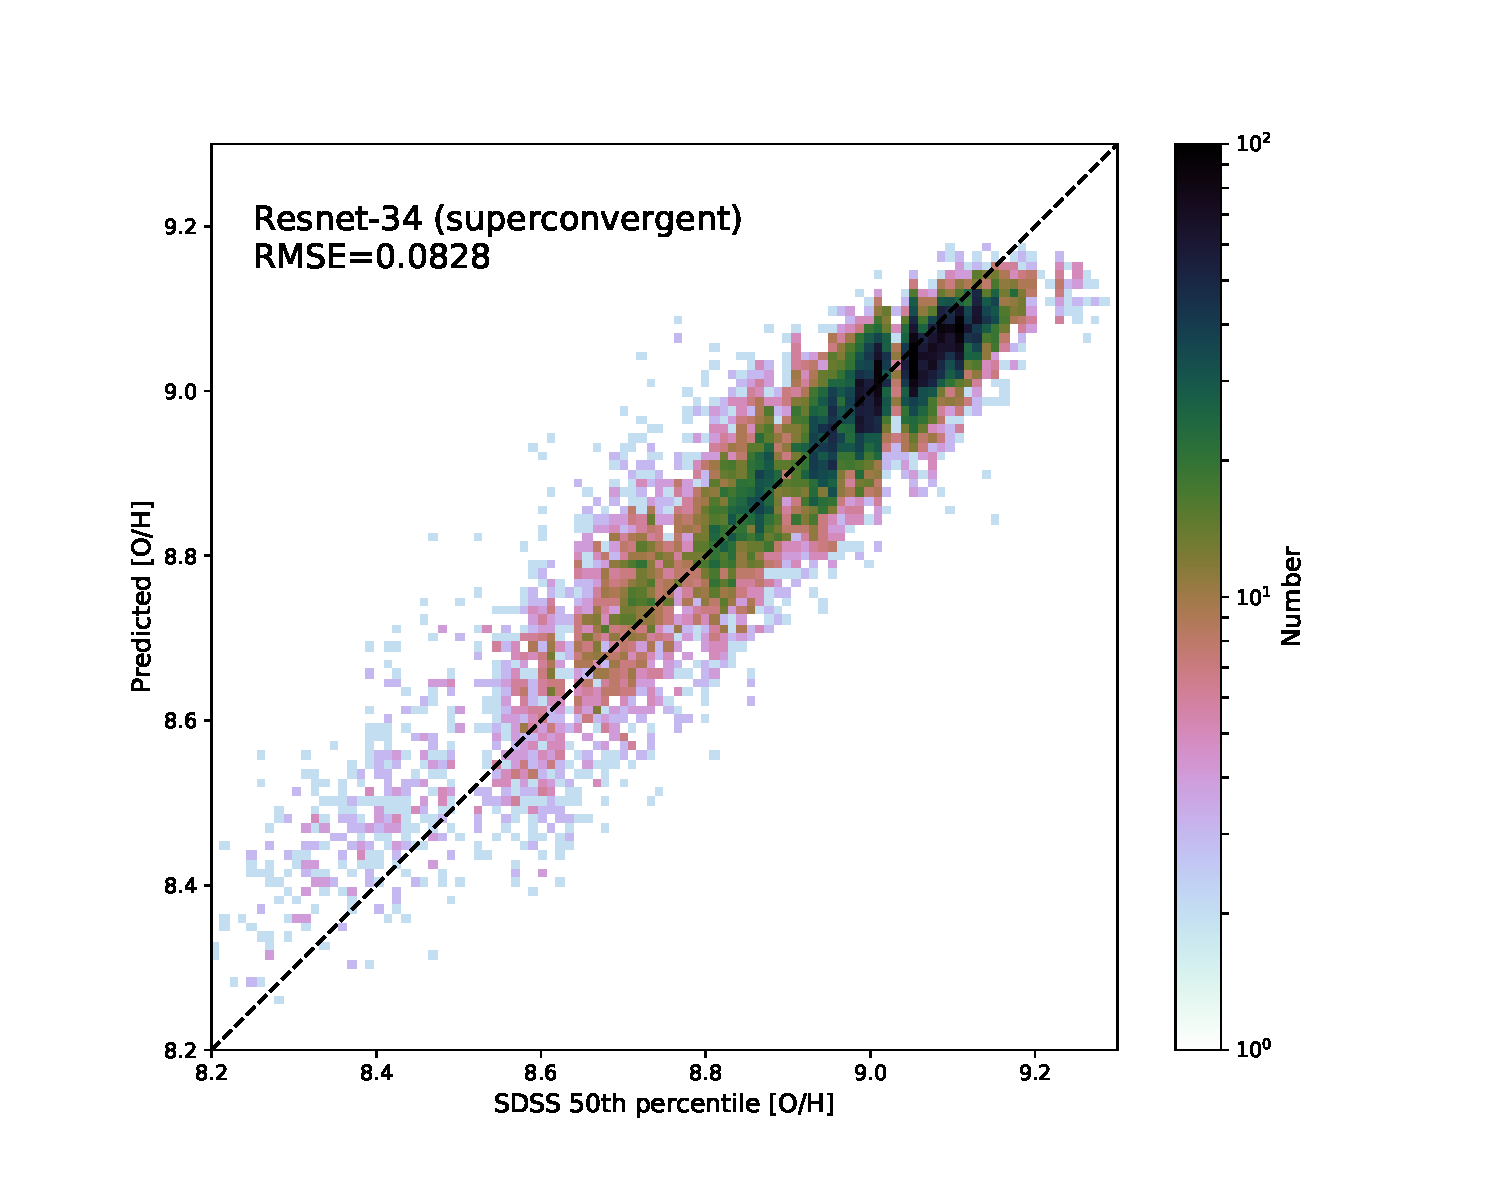
\includegraphics[width=\columnwidth]{superconvergent-resnet34_pred-vs-SDSS.pdf}
	\caption{\label{prediction-truth-plots}
		SDSS 50th percentile values for oxygen abundance derived from spectroscopy versus trained predictions for a variety of machine learning methods.
		(Upper) 34-layer Resnet predictions using only \textit{r}-band imaging.
		(Center) Random forest predictions using only \textit{gri} photometry.
		(Lower) 34-layer Resnet (super-convergent training) using \textit{gri} imaging.
		}
\end{figure}


%\begin{tabular}{l r  r r}
%	Method & & \textit{gri} & \textit{r}-band \\
%	\hline
%	\underline{[O/H] 50th percentile} \\
%	Resnet-34  &  & ??? & \textbf{0.1586} \\ 
%	Resnet-34 (5-fold) &  & \textbf{0.0835} & 0.143  \\
%	Resnet-34 (superconvergent)  &  & \textbf{0.0828} & ??? \\ 
%	%Resnet-101 & & 0.086 & 0.151 \\
%	Dieleman et al. CNN & & \\
%	Random decision forest & & \textbf{0.1356} & 0.260 \\
%	%TPOT & & 0.165 & 0.235 \\
%	Iyer et al. SED fitting & & 0.203 & 0.300 \\
%	Random sampling & & 0.265 & 0.265 \\
%	%\vspace{1em} \\
%	%\underline{$\log M_*/M_\odot$ 50th percentile} \\
%	%Resnet-34 & & 0.223 & 0.210 \\
%	note: also add training
%\end{tabular}



\subsection{Diagnostics}\label{sec:diagnostics}
Note by the way that our CNN trained on color images is able to predict better than by using only photometry (via random forest) and morphology ($r$-band CNN) independently.
Perhaps this is due to the fact that morphology is correlated with stellar population age or something else.
Color tells us the fundamental plane of SFR-$M_*$-metallicity but is biased by age and dust.

\subsection{Comparisons to Previous Works}\label{sec:previous work}
Lorem ipsum dolor sit amet, consectetur adipisicing elit, sed do eiusmod tempor incididunt ut labore et dolore magna aliqua. Ut enim ad minim veniam, quis nostrud exercitation ullamco laboris nisi ut aliquip ex ea commodo consequat. Duis aute irure dolor in reprehenderit in voluptate velit esse cillum dolore eu fugiat nulla pariatur. Excepteur sint occaecat cupidatat non proident, sunt in culpa qui officia deserunt mollit anim id est laborum.

Obviously compare with Huertas-Company et al.
Also look at Viviana's work as benchmark.
Compare with Galaxy Zoo as well.
Maybe CMU Deeplens paper for finding Einstein rings/arcs.
Note work from Sara Ellison's group: 
2016MNRAS.455..370E, 2017MNRAS.464.3796T, 2016MNRAS.457.2086T 

%\section{Discussion} \label{sec:discussion}


%\subsection{How important is morphology relative to color?}
%If the variance were to \textit{independently} scale with contributions from morphology and multiple photometric bands, then we would expect the MSE (\textit{or wait, actually the variance?}) to decrease like:
%\begin{equation}
%	{\rm MSE_{\rm gri}^{-1}} \approx {\rm MSE_{\rm photo}^{-1} + MSE_{\rm u}^2 + MSE_{\rm r}^2 + + MSE_{\rm r}^2}
%\end{equation}
%Actually, more properly:
%\begin{eqnarray}
%	\sigma_{\rm gri}^{-2} = \sigma_{\rm photo}^{-2} + \sigma_{\rm g}^{-2} + \sigma_{\rm r}^{-2} + \sigma_{\rm i}^{-2} 
%	- \left (\rho_{\rm gr}\sigma_{\rm g}\sigma_{\rm r}\right )^{-1} \nonumber\\
%	- \left (\rho_{\rm gi}\sigma_{\rm g}\sigma_{\rm i}\right )^{-1}
%	- \left (\rho_{\rm ri}\sigma_{\rm r}\sigma_{\rm i}\right )^{-1},
%\end{eqnarray}
%where we have assumed that $g$, $r$, and $i$ images are correlated with correlation coefficients given by $\rho$.
%We may actually be able to estimate $\rho$ by taking pairwise cross-correlations of different band images, e.g.,
%\begin{equation}
%\rho_{\mu \nu} = \frac{I_\mu \star I_\nu }{\sqrt{\left (I_\mu \star I_\mu \right ) \left (I_\nu \star I_\nu\right )}}.
%\end{equation}
%Here I have represented a correlation using the $\star$ symbol.
%
%
%\textbf{Also do:} Compare $r$-band vs. $gr$ (two-color) vs. $gri$ three-color imaging.

\section{The mass-metallicity relation} \label{MMR}
Given the low scatter in metallicity residuals (predicted $-$ true), we consider if the CNN is able to accurately predict stellar mass, and then leverage the mass-metallicity relation (MMR; Tremonti et al. 2004) to infer metallicity.
Alternatively, if SFR and $M_*$ are learned, then the fundamental metallicity relation (FMR; Mannucci et al. 2010, Lara-Lopez et al. 2010) may explain low residuals.


If there existed a fourth parameter, perhaps morphological in nature, then the marginalized MMR or FMR over particular values of this fourth parameter should be an even tighter relationship.
Such a result would be analogous to how the MMR at any controlled star formation rate (SFR) has smaller scatter than over all SFRs.

We find that the MMR constructed using SDSS-measured metallicity (via $R_{23}$) and the MMR constructed using CNN-predicted metallicity (from \textit{gri} imaging) are quantitatively different.
In both cases we have used the GalSpecExtra catalog for stellar masses.
The MMR using CNN metallicity has smaller scatter, where the weighted average ratio of scatter is NMAD(CNN)/NMAD(SDSS)~$= 0.821 \pm 0.077$.


We also produced plots of the MMR using SDSS- and CNN-predicted masses, and SDSS metallicity from the GalSpecExtra catalog.
Here the scatter in metallicity at given mass is again lower when using CNN predictions than for SDSS measurements.
The scatter is smaller by a factor NMAD(CNN)/NMAD(SDSS)~ $= 0.811 \pm 0.057$.

It is possible that the metallicity depends on some morphological component in addition to the emission lines informing the spectroscopic measurement.
However, we believe that the qualitatively accurate MMR is actually artifact of the CNN's limitations rather than its strengths.
Instead of finding a more fundamental representation of metallicity, the CNN likely detects the stellar mass.
In the case of using our CNN to predict metallicity, the slope of the MMR is shallower than from the ``true'' data. 
However, when the CNN is used to predict mass, the slope of is too steep.
This effect is driven by the fact that the CNN is unable to predict the full range of metallicities or masses, since the fraction of training examples at extremely low or high values is small.
\textbf{Therefore, the scatter in all of its predictions is narrower, such that when it predicts metallicity, the truncated range forces the MMR relationship to appear shallower, and when the CNN predicts $M_*$, the limited range in mass cause the MMR relationship to appear steeper.}

Why then does the MMR hold at all?
For if the CNN predicts, e.g., too narrow a distribution of metallicity, then what prevents those predictions from scattering over the full range in stellar mass?
The answer is quite possibly that the CNN only ``sees'' the metallicity via the stellar mass, such that the predicted MMR is effectively a relationship between the predicted mass and the true mass.
This theory is bolstered marginally by the fact that the fraction scatter for predicting mass is lower than for predicting metallicity (albeit not significantly so).
More intuitively, we might believe that the CNN can ``see'' that read and dead elliptical galaxies are higher in stellar mass, and that blue irregulars are lower in stellar mass.
Then the CNN simply needs to propagate the mass prediction through the tight $\sim 0.1$~dex MMR.

\textbf{How then can we achieve a NMAD~=~0.067~dex in metallicity by noisily propagating a signal with NMAD~=~0.22 scatter through the MMR which has 0.1~dex intrinsic scatter (Tremonti et al. 2004)?}

M/L ratio of redder galaxies are higher at fixed luminosity (Bell \& de Jong 2001; Kauffman+03).


\begin{figure}
	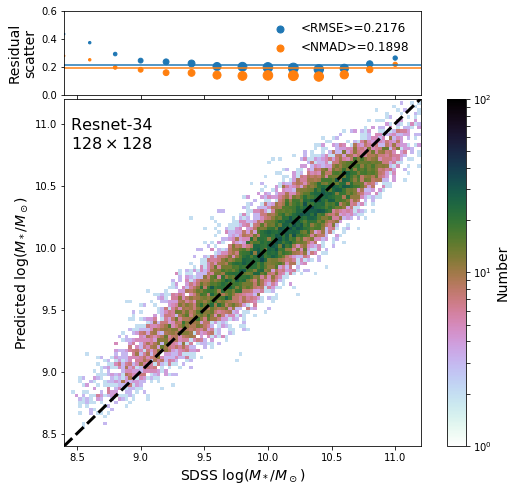
\includegraphics[width=\columnwidth]{predicted-vs-true-mass.png}
	\caption{\label{fig:predicting-mass}
		Same as Figure~\ref{fig:predicting-metallicity}, except that stellar mass predictions and truths are being compared (citation?).}
\end{figure}



%\subsection{Can stellar population age explain some of the scatter in the FMR?}

%\subsection{Why do CNNs work so well at predicting spectroscopic quantities?}
%Can we find a non-CNN parameter or method of explaining the scatter?

\section{Future Applications}\label{sec:future}
Lorem ipsum dolor sit amet, consectetur adipisicing elit, sed do eiusmod tempor incididunt ut labore et dolore magna aliqua. Ut enim ad minim veniam, quis nostrud exercitation ullamco laboris nisi ut aliquip ex ea commodo consequat. Duis aute irure dolor in reprehenderit in voluptate velit esse cillum dolore eu fugiat nulla pariatur. Excepteur sint occaecat cupidatat non proident, sunt in culpa qui officia deserunt mollit anim id est laborum.

\section{Summary}\label{sec:summary}
Lorem ipsum dolor sit amet, consectetur adipisicing elit, sed do eiusmod tempor incididunt ut labore et dolore magna aliqua. Ut enim ad minim veniam, quis nostrud exercitation ullamco laboris nisi ut aliquip ex ea commodo consequat. Duis aute irure dolor in reprehenderit in voluptate velit esse cillum dolore eu fugiat nulla pariatur. Excepteur sint occaecat cupidatat non proident, sunt in culpa qui officia deserunt mollit anim id est laborum.

Our main conclusions are the following:
\begin{enumerate}
	\item Lorem ipsum dolor sit amet, consectetur adipisicing elit, sed do eiusmod tempor incididunt ut labore et dolore magna aliqua. Ut enim ad minim veniam, quis nostrud exercitation ullamco laboris nisi ut aliquip ex ea commodo consequat. Duis aute irure dolor in reprehenderit in voluptate velit esse cillum dolore eu fugiat nulla pariatur. Excepteur sint occaecat cupidatat non proident, sunt in culpa qui officia deserunt mollit anim id est laborum.

	\item Lorem ipsum dolor sit amet, consectetur adipisicing elit, sed do eiusmod tempor incididunt ut labore et dolore magna aliqua. Ut enim ad minim veniam, quis nostrud exercitation ullamco laboris nisi ut aliquip ex ea commodo consequat. Duis aute irure dolor in reprehenderit in voluptate velit esse cillum dolore eu fugiat nulla pariatur. Excepteur sint occaecat cupidatat non proident, sunt in culpa qui officia deserunt mollit anim id est laborum.
\end{enumerate}

\section*{Acknowledgements}
\editorial{The authors also wish to thank the anonymous referee whose comments and suggestions significantly improved both the quality and clarity of this work.}
The authors also thank David Shih and Matthew Buckley for use of their GPU cluster at Rutgers University High Energy Experimental Physics department. %, and Kartheik Iyer for providing SED fits as benchmark as well as for valuable discussion.
This research made use of the {\sc IPython} package \citep{Perez2007} and {\sc matplotlib}, a Python library for publication quality graphics \citep{Hunter2007}. Funding for the SDSS and SDSS-II has been provided by the Alfred P. Sloan Foundation, the Participating Institutions, the National Science Foundation, the U.S. Department of Energy, the National Aeronautics and Space Administration, the Japanese Monbukagakusho, the Max Planck Society, and the Higher Education Funding Council for England. The SDSS Web Site is \url{http://www.sdss.org/}.

%%%%%%%%%%%%%%%%%%%% REFERENCES %%%%%%%%%%%%%%%%%%
% The best way to enter references is to use BibTeX:
\bibliographystyle{apj}
\bibliography{master} % if your bibtex file is called example.bib

%%%%%%%%%%%%%%%%% APPENDICES %%%%%%%%%%%%%%%%%%%%%
\appendix
%
\section{Residual convolutional neural networks}
%
% If you want to present additional material which would interrupt the flow of the main paper,
% it can be placed in an Appendix which appears after the list of references.

In general, CNNs become difficult to train after many layers are added.
We select an architecture called a residual neural network, or \textit{resnets} (He et al. 2015), which contains enhanced ``shortcut connections'' but are otherwise similar to other CNNs.
Resnets have been shown to continue learning with increasing depth without the added cost of extra parameters.
This is likely because the network has already found the best representation possible at a shallower layer, and further layers simply noisily propagate the same signal and degrade the loss.
Therefore resnets are able to learn deep representations of the data.

We find that a 34-layer resnet (Resnet-34) architecture can be trained efficiently on a Pascal P100 with 16~GB of memory.
Using the hyperparameters described below, an epoch takes about 60~seconds to train.
We initialize our resnet with pretrained weights from the ImageNet (Russakovsky et al. 2014; He et al. 2015) 1.7~million image data set trained to recognize 1000 classes of objects found on Earth (i.e., cats, dogs, or cars).
In practice, the filters learned through the early layers of the pretrained CNN can be used for other image recognition tasks, aptly named ``transfer learning'' (cite).


\subsection{Hyperparameter selection}

\subsection{Data augmentation}
Nearly all neural networks benefit from larger training samples because they help prevent overfitting.
Outside of the local Universe, galaxies are seen at nearly random orientation; such invariance permits synthetic data to be generated from rotations and flips of the training images.
Each image is fed into the network along with four augmented versions, thus increasing the total training sample by a factor of five.
%Additional small zooms of $< 5\%$ may also be applied to enlarge the training size.
This technique is called data augmentation, and is particularly helpful for the network to learn uncommon or unrepresented truth values (e.g., in our case, very metal-poor or metal-rich galaxies).
Each training-augmentation is fed-forward through the network and gradient contributions are computed together as part of the same mini-batch.
A similar process is applied to the network during predictions, which is called test-time augmentation (TTA).
Synthetic images are generated according to the same rules applied to the training data set. 
The CNN predicts an ensemble average over the augmented images.
It has been found that data augmentation improves predictions by as much as $\sim 20\%$ (cite).

\subsection{Cyclical learning rate annealing}
The learning rate determines how large of a step each network weight takes in the direction of the backpropagated error.
A large learning rate thus forces the weights to make large updates, which generally prevents overfitting but also may cause the parameters to overshoot minima in the loss function landscape.
A small learning rate may allow the weights to get stuck in a local minima near their initial positions, or also might cause the network to learn very slowly.
The number of local minima increases exponentially with dimensionality (cite), so selecting a low learning rate does not ensure that the network will eventually make it to near the global minimum.
Therefore, it is often useful to anneal, or reduce, the learning rate from a high value in the beginning -- which allows the weights to find the right ballpark values -- to a low value -- which allows the weights to take finer steps near the global minimum -- over the course of multiple training epochs.

In practice, annealing can be enforced manually, e.g., the learning rate might be reduced by a factor of 10 every time the loss function plateaus over a number of epochs.
Eventually even reduced learning rates do not permit additional improvement of the loss, and so the training period is concluded.
We instead use a method called cosine annealing, during which the learning rate is annealed continuously over one or more epochs for \textit{each} mini-batch until it eventually reaches zero.


We employ stochastic gradient descent with restarts (SGDR), over progressively longer training cycles, and restart cosine annealing over each cycle (Leslie Smith 2015?). 
For example, the first cycle comprises one epoch during which the learning rate is cosine annealed.
It then trains for another cycle with cosine annealing, which starts at the same learning rate but is annealed over twice the duration (two epochs).
These ``restarts'' have been shown to kick the weights configuration out of saddle points in the loss of some high-dimensional parameter space.
Training can then proceed past what appear to be local minima but are actually saddle points (where gradient descent generally performs poorly).


\subsection{Layer learning rates}
ADD MORE HERE

Frozen training to get final activates in right ``ballpark.''
We then unfreeze all layers and train using different rates in different layer groups.

\subsection{Batch normalization and Dropout}

Batch normalization (BN; 1502.03167) is a technique developed to fix the vanishing gradients problem which make deep networks inefficiently slow to train.
The issue arises when gradients are backpropagated through deep neural networks to update weights, and loss contributions become vanishingly small except only when the weights have small magnitudes.
Normalizing the inputs to each mini-batch mean and standard deviation somewhat remedies the problem, and has been applied to (convolutional) neural networks since the 1990s.
BN extends this normalization to all activations in hidden layers, thus adding two hyperparameters which modulate the mean and standard deviation of each layer to zero and unity, respectively.
The BN hyperparameters are learned for each mini-batch and are updated in addition to weight parameters during the backward pass.
% if confused refer to  https://kratzert.github.io/2016/02/12/understanding-the-gradient-flow-through-the-batch-normalization-layer.html4

Without BN, activations in any given layer may span a large range and contributions from certain parts of the network may become dwarfed by others.
After the normalization step, all pre-activations are on the same scale and thus gradient descent steps can more efficiently traverse the loss function space.
Training proceeds more rapidly and converges toward a solution more quickly.
Choice of mini-batch size also impacts the learning rate, as small batch size increases stochasticity in each gradient.
Large batch size allows for better parallelization on the GPU and ensures smoother gradients.
We note that smooth gradients across mini-batches can prevent the solution from hopping out of local basins, and negatively impact performance.
Increasing the learning rate as batch size is increased can resolve this problem, at least in part, but limits the convergence ability of the network (until the rate is annealed).
We find in practice that batch sizes between 128 and 512 work best at balancing noisy gradients and learning rate.


Dropout is a method of disabling a random subset of connections after linear layers for each mini-batch (Hinton et al. 2012).
By removing random connections between fully-connected layers, dropout effectively treats each mini-batch as one in an ensemble of random training subsets .
It is instructive to think of each mini-batch in the full training data as analogous to a decision tree in a random forest.
The ensemble of learned gradients is less prone to overfit the training data set because the network is forced to discard random (and potentially valuable) information.
The resulting network is better able to, for example, learn subtle differences in the data that would otherwise be ignored when more obvious features dominate the gradient descent process.
Since our Resnet architecture is broadly separated into multiple groups of layers, we can apply lower dropout rate at earlier layers in order to ensure that those filters are learned more quickly.
Using a differential dropout rate is sensible because filters learned in the first few layers of the network tend to be Gabor filters and edges in general, and there is little risk of overfitting when such low-level abstractions are always necessary for learning high-level features in the middle and final layers.

During validation and testing, dropout is not used because all of the data is useful for predictive power.
We use dropout rates of 0.25 for the linear layer after the early group, and 0.50 at the later linear layer.
We find that dropout combined with BN -- although not recommended in the original paper -- work in tandem to boost training speeds and avoid overfitting.



% Don't change these lines
\bsp	% typesetting comment
\label{lastpage}
\end{document}
